\documentclass[17pt]{flash}
\usepackage{tkz-euclide}
\startdatakeys
\cycle{}
\connaissancesRequises{}
\competencesTravaillees{}
\enddatakeys
\begin{document}

\flashvisibletimertrue
\FlashSetItemSep{80pt}
\FlashSetVtop{-4em}
\FlashSetTitle{Théorème de Pythagore}

\FlashShowConsignes{%
        \item Le triangle suivant est-il rectangle~? Démontrer votre affirmation.
}

\small
\flash{180}{%
    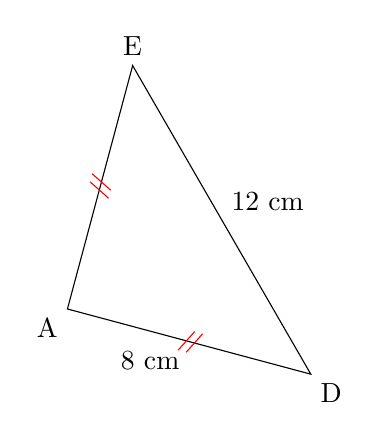
\begin{tikzpicture}[scale=0.4,rotate=-15]
        \coordinate[label=below left:A](A)at(0,0);
        \coordinate[label=below right:D](D)at(8,0);
        \coordinate[label=above:E](E)at(0,8);
        \draw(A)--(D)--(E)--cycle;
        \tkzMarkSegments[mark=s||,color=red](A,D A,E)
        \path(A)--(D)node[midway, below left]{8 cm};
        \path(E)--(D)node[midway, above right]{12 cm};
    \end{tikzpicture}
}
\footnotesize
\FlashCorrection

\end{document}